\documentclass[12pt,a4paper]{scrreprt}

\usepackage{ucs}
\usepackage[utf8x]{inputenc}
\usepackage[T1]{fontenc}
\usepackage[ngerman]{babel}
\usepackage{graphicx}
\usepackage{listings}
\usepackage{color}

\usepackage[hidelinks]{hyperref}

% Festlegung Art der Zitierung - Havardmethode: Abkuerzung Autor + Jahr
\bibliographystyle{}

% Literatur Datei
\bibliography{literatur}


\begin{document}

%verändert die Schriftart der Überschriften
\setkomafont{disposition}{\normalcolor\bfseries}

\begin{titlepage}

\centering

\title{Praxissemesterbericht \\  
\vspace{1cm} \large zu \\ 
\vspace{1cm}  Fuzzing mit American Fuzzy Lop \\
\vspace{0.5cm} bei der Firma \\
\vspace{0.5cm} Airbus DS Optronics GmbH \vspace{1.5cm}}


%\vspace{1.5cm}

\author{Andreas Eisele}

\vspace{1.5cm}

\date{\today{}, Aalen}
\maketitle
\end{titlepage}


\tableofcontents

\newpage
\renewcommand{\thesection}{\arabic{section}}


\chapter{Praxisstelle und Klausel}



\begin{minipage}{1\textwidth}

\textbf{Airbus Defence \& Space Optronics GmbH} \\
Carl-Zeiss-Straße 22 \\
73447 Oberkochen

\vspace{2cm}

\textbf{Betreuer \& Abteilung} \\
Michael Adam, Softwareentwicklung (Sensor-Architektur) \\


\vspace{0.5cm}

\textbf{email}:  michael.adam@airbusds-optronics.de \\
\textbf{phone}: 07364 9557 - 122
	

\end{minipage}

\vspace{3cm}

\begin{minipage}{1\textwidth}

Hinweis zur Weitergabe bzw. Verwendung von ....

\end{minipage}



\newpage
\chapter{Eidesstattliche Erklärung}


\begin{minipage}{0.99\textwidth}

Hiermit erkläre ich, \textbf{Andreas Eisele}
dass ich die vorliegenden Angaben in diesem Bericht
zu meinen Tätigkeiten im Praxissemester bei
Airbus DS Optronics GmbH
wahrheitsgetreu und selbständig verfasst habe.
Weiterhin versichere ich, keine anderen als die angegebenen Quellen und Hilfsmittel benutzt zu haben, dass alle Ausführungen, die anderen Schriften wörtlich oder sinngemäß entnommen wurden, kenntlich gemacht sind und dass die Arbeit in gleicher oder ähnlicher Fassung noch nicht Bestandteil einer Studien- oder
Prüfungsleistung war. (Soweit mir bekannt!)

\vspace{2cm}

\end{minipage}

\begin{minipage}{0.99\textwidth}

Ort,  Datum \hspace{3cm} Unterschrift (\textbf{Student})

\end{minipage}

%---------------------------------------------------------------

\vspace{3cm}

\begin{minipage}{0.99\textwidth}

Bestätigung der inhaltlichen Richtigkeit:
Der vorliegende Bericht wurde durch den zuständigen Betreuer
\textbf{Michael Adam} korrekturgelesen und auf inhaltliche Korrektheit geprüft.

\vspace{2cm}

\end{minipage}


\begin{minipage}{0.99\textwidth}

Ort, Datum \hspace{3cm} Unterschrift (\textbf{Betreuer})

\end{minipage}


\newpage
\chapter{Kurzfassung}
Im Rahmen dieser Arbeit ....


\newpage
\chapter{ Motivation und Ziel der Arbeit  }

\section{Motivation}

Das testen von Software ist einer der wichtigsten Entwicklungsschritte eines jeden Software-Entwicklungsmodells. 

Oftmals ist die Testphase einem erhöhten Zeitdruck ausgesetzt und demzufolge wird sie nicht selten in einem verkürzten Rahmen durchgeführt.
Das hat zur Folge, dass nicht selten Fehler in Software enthalten sind, die mit entsprechenden Anstrengungen beziehungsweise einem guten Testverfahren hätten gefunden werden können. Dabei ist der Aspekt ein qualitativ gutes Produkt zu liefern genauso wichtig, wie der Prävention von Schwachstellen, die von Cyber-Kriminellen ausgenutzt werden könnten. 

Mit Fuzzer Programmen hat sich eine Testmethode etabliert, die weitaus mehr Testfälle abdecken kann und dies in deutlich kürzerer Zeit als das mit herkömmlichen Testverfahren möglich ist.
Insbesondere die jüngsten Fuzzer Tools sind oft vielseitig einsatzfähig und werden immer attraktiver in der Handhabung.



\section{Ziel der Arbeit}

Mit diesem Pilotprojekt soll getestet werden, ob sich einer der heutzutage populärsten Fuzzer zum einen gut in den Testprozess einbinden lässt und zum anderen ob die Ergebnisse der Testläufe auch den Erwartungen entsprechen.

Zudem soll die Frage geklärt werden, wie portabel der Fuzzer auf unterschiedlichen Zielsysteme ist und wenn möglich in Entwicklungsumgebungen einbinden lässt. 


\chapter{Vorgehen}

\begin{itemize}

\item \textbf{Kennenlernen von AFL} - Um einen Fuzzer anzuwenden ist es notwendig zuerst auch dessen Funktionsaufbau- und Umfang zu erforschen. Die Dokumentation zu AFL ist ausführlich setzt aber auch Entwicklungserfahrung und ein tieferes Verständnis der C basierten Programmiersprachen voraus, da er in erster Linie für solche Anwendungen entwickelt wurde. Die Recherche im Web nach Tutorials oder Vorstellungen von AFL helfen Anfänger sehr sich in die Materie einzuarbeiten, da hier auch Beispiele für Neulinge zu finden sind.

\vspace{1cm}

\item \textbf{Tests mit Beispielprogrammen} - Unverzichtbar wenn man neu in das Thema einsteigt, ist es AFL anhand selbst geschriebener kleiner Beispielprogrammen zu testen. Durch das einbauen von Fehlern in die Testprogramme erhält man zudem ein besseres Verständnis des Fuzzers.

\vspace{1cm}

\item \textbf{Kennenlernen der Zielsoftware} - Ein genauso wichtiger Punkt ist es die Zielsoftware zu kennen. Auch wenn es grundsätzlich nicht notwendig ist um das Ziel zu testen, so ist es vor allem dann wichtig das Ziel-Programm zu kennen, wenn die gefundene Schwachstelle auch behoben werden soll.

\vspace{1cm}

\item \textbf{Aufbau von Testumgebung} - Abhängig davon, ob das Ziel ohne Anpassungen direkt getestet werden kann ist es unter Umständen notwendig erst einmal eine Testumgebung zu implementieren. Hier sollen dann Daten für AFL mitgeschnitten werden und in passenden Testfällen eingesetzt werden.

\vspace{1cm}

\item \textbf{Testen und Evaluation} - Nachdem die Tests vorbereitet sind können die Fuzzing-Sessions beginnen. Wenn die Testläufe durchlaufen sind, ist es wichtig sich zu vergewissern das die Tests auch eine zur Komplexität des Programms beziehungsweise der Komponente passende Abdeckung erreicht haben. Sollten Programmhänger- oder Abstürze aufgetreten sein so kann anhand des Output` s von AFL mittels Debugging die Stelle im Quellcode gefunden werden.

\end{itemize}


\newpage
\chapter{Grundlagen} 

\section{Fuzzing}
Fuzzing auch als "Robustheits - Test" bekannt, ist eine Methode um Software auf Stabilität und Schwachstellen zu testen. 

Im Vergleich zu Unit-Tests, bietet Fuzzing ein weitaus größeres Spektrum an generierten Zufallsdaten, welche auf die Zielschnittstellen ausgeführt werden. 
Da die Daten von dem entsprechenden Fuzzing-Programm generiert werden , sind diese unabhängig und werden nicht von den Entwicklern beeinflusst. Das grundlegende Prinzip von Fuzzing ist damit das "beschießen" der Zielsoftware mit generierten Zufallsdaten und so zu überprüfen, ob sich das Programm unerwartet verhält und dadurch eine Schwachstelle aufgetreten ist.

Als unerwartetes Verhalten ist in der Regel das hängen oder abstürzen einer Software gemeint. Diese "Bugs" haben als Ursache oft Speicherleks, welche häufig in den Sprachen C und C++ auftreten, da diese dort nicht bereits automatisiert abgefangen werden. Die Schwachstellen, welche durch so einen Bug auftreten können, sind oft auch Ziel von Kriminellen die insbesondere bei sensibler Software wie Kommunikationsprogrammen hier schaden anrichten können.

Das erste mal wurde der Begriff Fuzzing und diese Methode zu testen von Barton Miller und seinen Studenten an der University of Wisconsin-Madison 1989 entwickelt.
Viele Jahre konnte sich Fuzzing für den breiten Gebrauch nicht etablieren. Aufgrund von sehr aufwendigen Anpassungen die notwendig waren um die damaligen Fuzzer-Tools auf die entsprechende Zielsoftware zuzuschneiden waren diese für die Testphase schlicht zu kostenintensiv. 

In den letzten Jahren hat durch die Entwicklung effizienterer Tools das Thema Fuzzing eine deutlich höhere Verbreitung erfahren. Besonders einer dieser Fuzzing-Programme wird im Rahmen dieser Arbeit behandelt.   

\newpage

\section{American Fuzzy Lop}
Der Fuzzer AFL wurde 2014 von Michal Zalewski einem Google Mitarbeiter entwickelt. Im Vergleich zu anderen verfügbaren Fuzzing-Tools unterscheidet sich American Fuzzy Lop maßgeblich, durch dessen neuen Ansatz mit einem genetischen instrumenten-geführten Algorithmus. Die Resultate von Tests mittels Fuzzing haben sich durch den Einsatz mit AFL signifikant verbessert und so zu dessen Bekanntheit geführt. 
Dieses Fuzzer-Programm ist in der Lage sowohl Black-Box als auch White-Box Tests durchzuführen und ist als freie Open-Source-Software unter der Apache Version 2 Lizenz verfügbar. 

Es zeichnet sich insbesondere durch die Instrumentierung während des Kompilierprozesses aus und erreicht dadurch eine sehr hohe Pfadabdeckung des Ziels. Indem Instruktionen in den Assembler-Code geschrieben werden, ist AFL in der Lage auf Veränderungen die im Ziel-Programm ausgelöst werden zu erfassen und darauf zu reagieren.
Eine weitere Besonderheit sind die Mutationen auf die Sample-Dateien. Um überhaupt fuzzen zu können muss mindestens eine minimale valide Datei vorliegen, welche von dem zu testenden Porgramm verarbeitet wird. Diese Dateien werden in einer Queue gespeichert und fortlaufend modifiziert oder verworfen. Wenn eine dieser Veränderungen einen neuen Programzustand verursacht wird diese Datei in die Queue mit aufgenommen.

Dieser Prozess wird immer wieder wiederholt, bis alle möglichen Programpfade mit den mutierten Dateien in der Zielsoftware durchlaufen wurden.



\begin{figure}[htbp] 
  \centering
     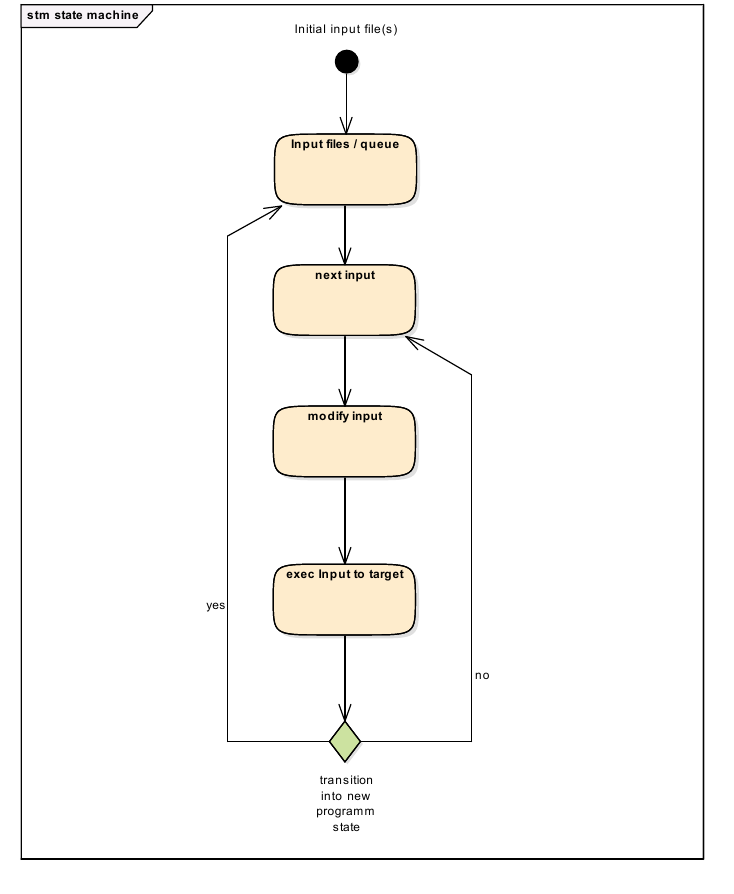
\includegraphics[width=0.75\textwidth]{state_machine.png}
  \caption{AFL State-Machine}
  \label{fig:Bild0}
\end{figure}




\subsection{Welche Software kann mit AFL getestet werden?}
AFL wurde in erster Linie für Programme entworfen, die Dateien verarbeiten oder über Stdin Eingaben erhalten. Da die Architektur von AFL bedingt Dateien auf die zu testende Software auszuführen.

Sollte dies nicht auf die Zielsoftware zutreffen, kann es trotzdem möglich sein diese mit AFL zu testen. Wichtig an dieser Stelle ist zum einen das speichern von Daten, die im Programm verarbeitet werden und an geeigneter Stelle in das Programm geführt werden. Das bedingt in vielen Fällen die Software in Komponenten aufzuteilen. 

% https://events.linuxfoundation.org/sites/events/files/slides/AFL%20filesystem%20fuzzing,%20Vault%202016_0.pdf

\newpage
\subsection{Instrumentierung}	

Während des Instrumentierungsschrittes setzt AFL Instruktionen in den Assemblercode anhand derer eine Tuple-Karte der Zielsoftware erstellt wird. Durch das setzen der AFL Flags bei betreten einer Funktion, einer Verzweigung oder Schleifen entsteht ein vollkommenes Bild des Ziels und ermöglicht dem Algorithmus so zu beurteilen wann ausreichend Durchläufe erfolgt sind.


\begin{figure}
\centering
	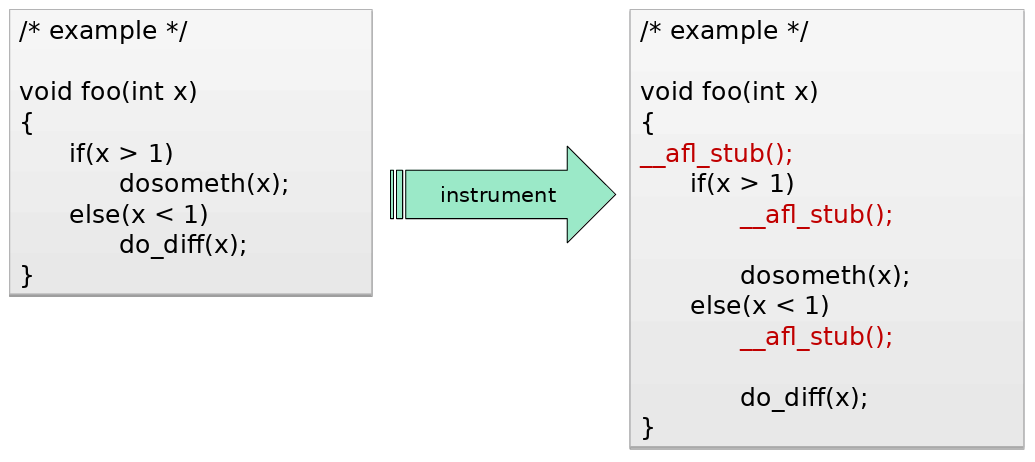
\includegraphics[width=1\textwidth]{instrument.png}
	\caption{Instrumentierung}

\end{figure}


\subsection{Erfassen neuer Programzustände}

Durch die im Instrumentierungsprozess erstellte Tupel-Karte ist es AFL möglich während der Fuzzing-Session sehr schnell vorherige bereits passierte Programmpfade anhand derer Tupelmenge mit dem aktuellen Pfad zu vergleichen und so den Wechsel in einen neuen Programmzustand zu detektieren. 
So wird zum einen erkannt ob durch das ausführen dieser Daten neue Programmpfade passiert wurden und wie oft diese Sequenz bereits durchlaufen wurde.

Sollte durch das ausführen einer mutierten Datei so ein neuer Programmzustand erreicht worden sein, wird diese Datei beibehalten und für weitere Mutationen in einer Queue gespeichert. Damit wird sicher gestellt, dass die Mutationen nur jeweils auf interessanten Dateien basieren und sich so in tiefere Programmschichten vorarbeiten können.

\newpage

*\textbf{Beispiele von Tuple-Sequenzen}*

\begin{itemize}

\item[1)] \textbf{A->B->C->D->E}	= erstellte Tupel (AB),(BC),(CD),(DE) \\ => neu entstandene Tupel: = erstellte Tupel

\item[2)] \textbf{A->B->C->A->E} = erstellte Tupel (AB),(BC),(CA),(AE) \\ => neu entstandene Tupel:  (CA),(AE)

\item[3)] \textbf{A->B->C->A->B->C->D->E} = erstellte Tupel (AB),(BC),(CA),(DE) \\ => es sind \textbf{KEINE} neuen Tupel hier entstanden

\end{itemize}

\vspace{1cm}

\subsection{Mutation}

Der Fuzzer wird unter Berücksichtigung der verfügbaren Sample-Dateien beginnend alle Dateien, die in der Queue gespeichert sind mutieren. Der Queue werden daraufhin weitere Dateien hinzugefügt die einen neuen Programmzustand verursacht haben. 

Dieser  Vorgang wiederholt sich solange bis keine neuen Programmpfade mehr durch die Mutationsschritte gefunden werden können.

\vspace{1cm}

\textbf{Die Mutation startet mit folgenden deterministischen Schritten:}

\begin{itemize}

\item flippen jeden Bits in der Datei, anschließend jedes Byte

\item aufteilen der Datei in 8, 16 und 32 Bit Teile und das ausführen von arithmetischen Operationen auf diese Teile

\item ersetzen von Bytes durch bekannte interessante Integer \(0, 1, INT\_MAX, etc\)    

\end{itemize}

Nach diesen Schritten folgen noch weitere zufällige Mutationen, welche die bereits aufgeführten wiederholen und zudem Daten von der Datei löschen und/ oder welche hinzufügen. 


\subsection{Fuzzing Session}

\subsection{Evaluation}

\section{mehr Grundlagen ......}

%-----------------------------------------------------------------

\newpage
\chapter{Fuzzing Session}

\section{Zielsoftware System-Stack}
Der System Stack ist die softwareseitige Lösung für die Kommunikation zwischen verschiedenen Aufnahmegeräten.

Ein Master-Stack kann mit mehreren Slave-Stack`s kommunizieren. Der Stack ist in mehrere Schichten aufgeteilt die über Schnittstellen miteinander verbunden sind. Im Einsatz ruft ein Device seinen Stack beziehungsweise die oberste Schicht auf um Daten zu übertragen und der Stack wiederum über seine unterste Schicht ein entsprechendes IO\_Device um die Daten zu übertragen.


\section{Aufteilung des Ziels in Schichten}

Wie in dem Abschnitt ....... angesprochen, ist Software die von sich aus nicht schon Dateien oder Stdin-Eingaben verarbeitet daraufhin anzupassen.

Im Falle des System-Stack wurden die einzelnen Schichten für sich oder teils mit darüber- oder darunterligenden Schichten geprüft. 



\newpage
\section{Mitschneiden von Programmdaten}

\begin{figure}[htbp] 
  \centering
     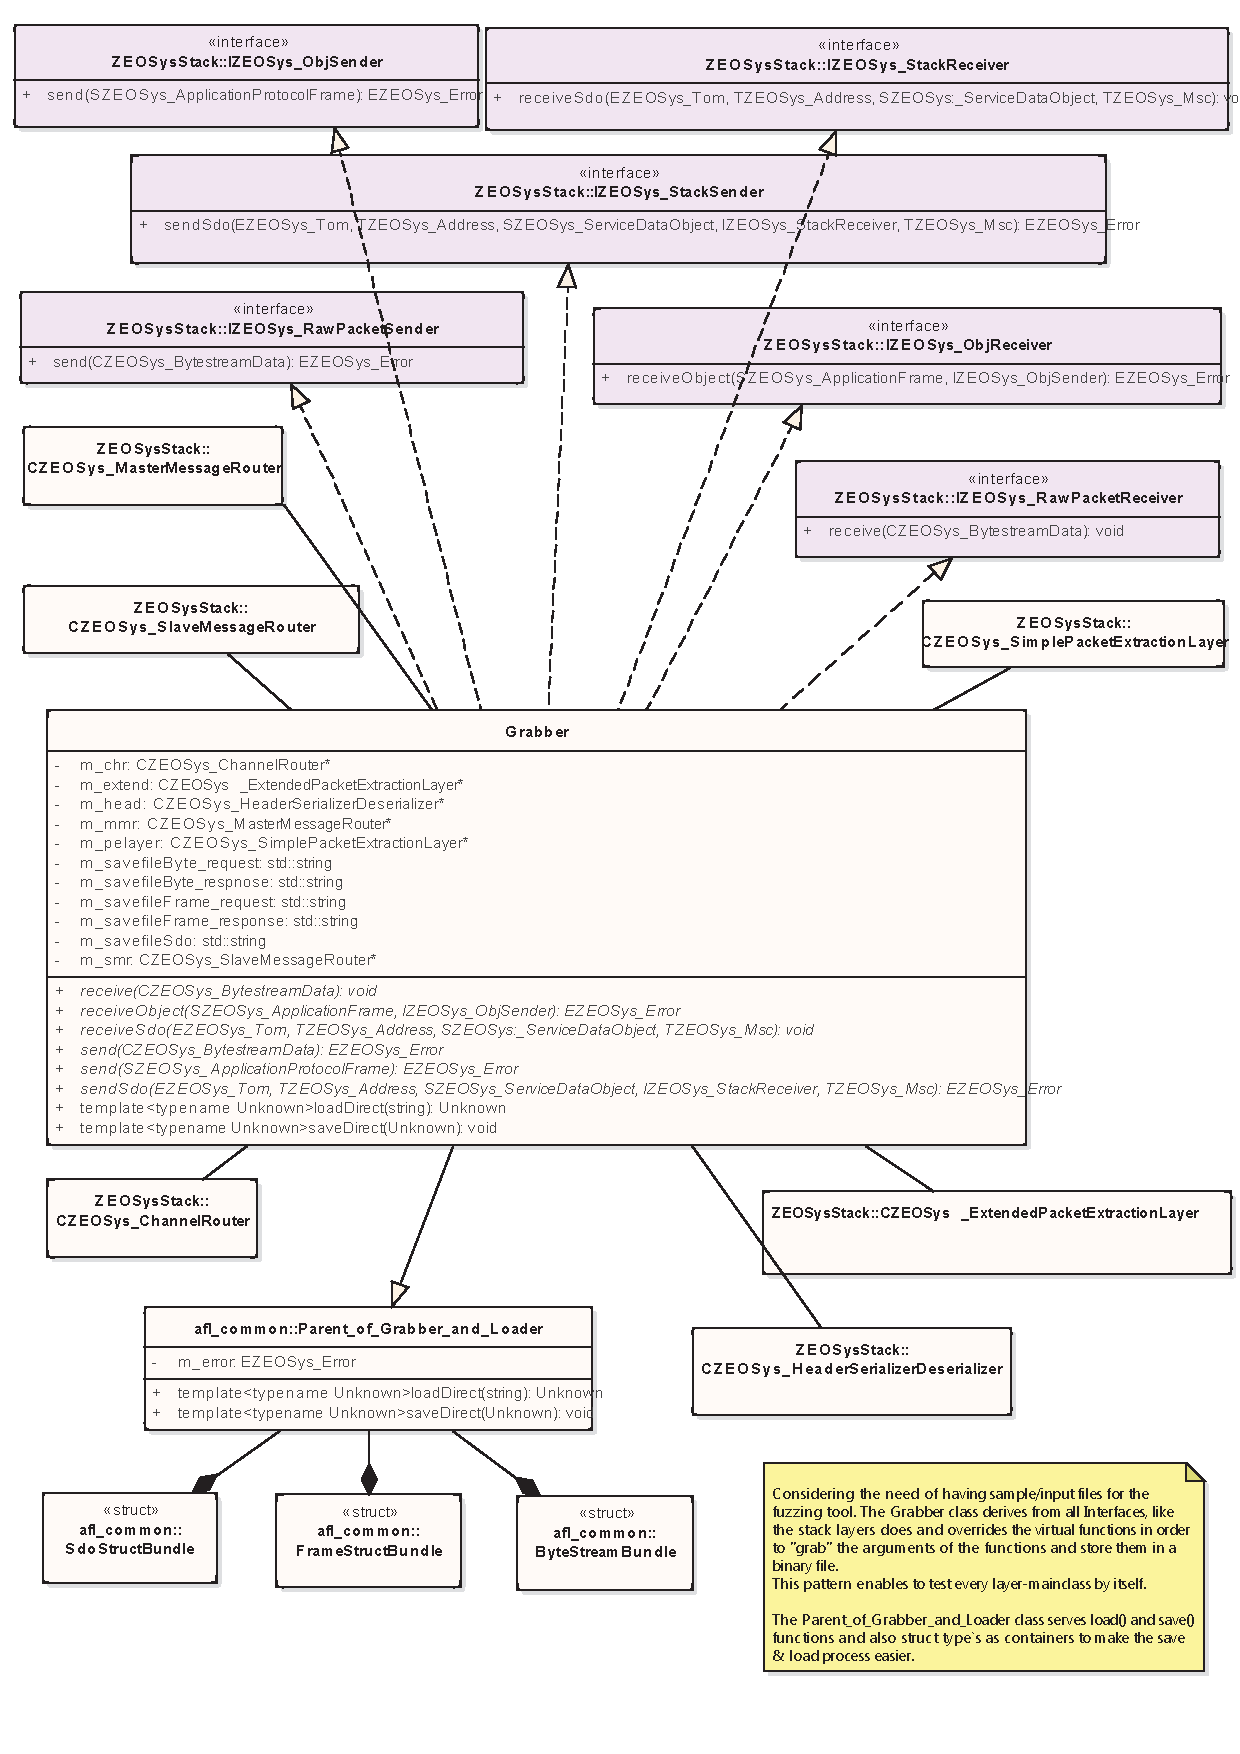
\includegraphics[width=1.0\textwidth]{generate.pdf}
  \caption{Grabber Klasse}
  \label{fig:Bild1}
\end{figure}


\begin{figure}[htbp] 
  \centering
     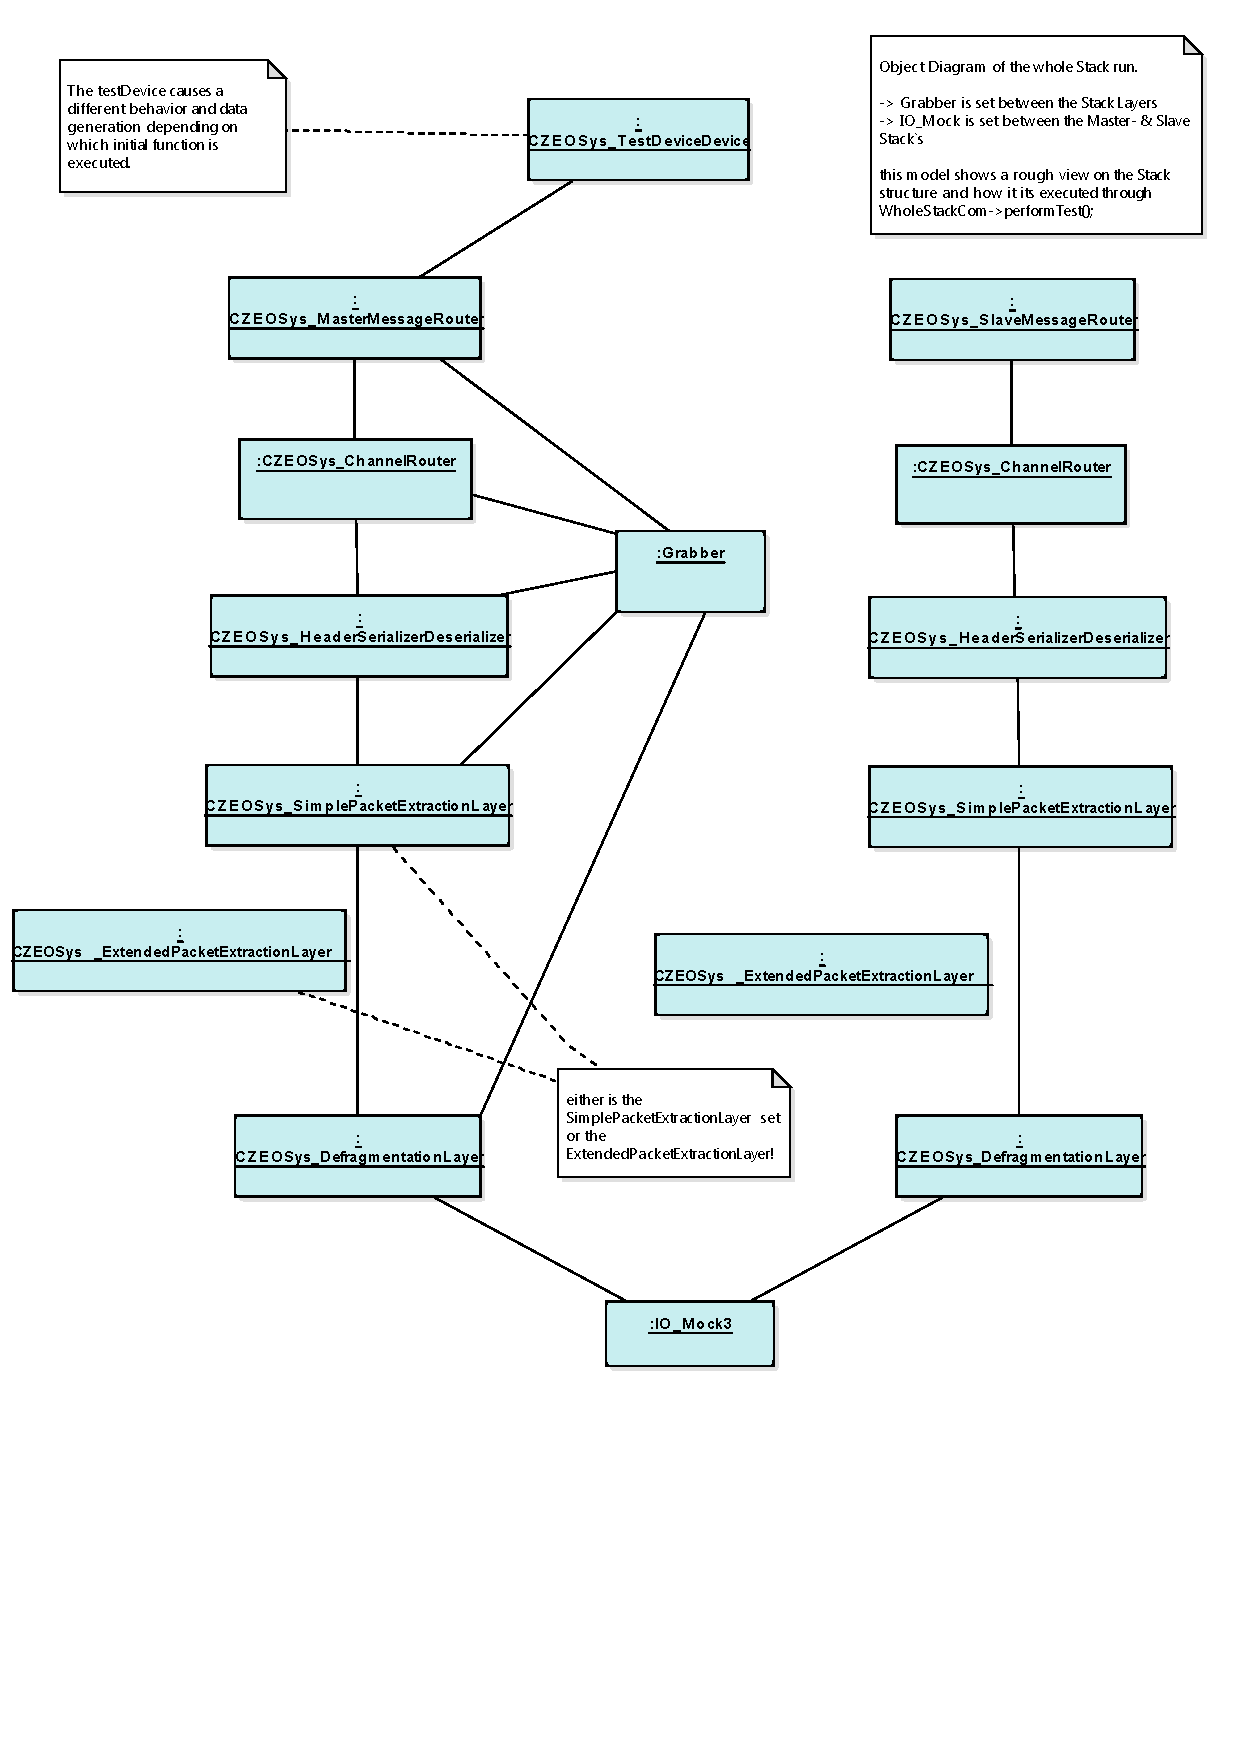
\includegraphics[width=1.0\textwidth]{object_diagramm.pdf}
  \caption{Einbettung Grabber}
  \label{fig:Bild2}
\end{figure}

\newpage
\section{Testumgebungen anlegen}

\begin{figure}[htbp] 
  \centering
     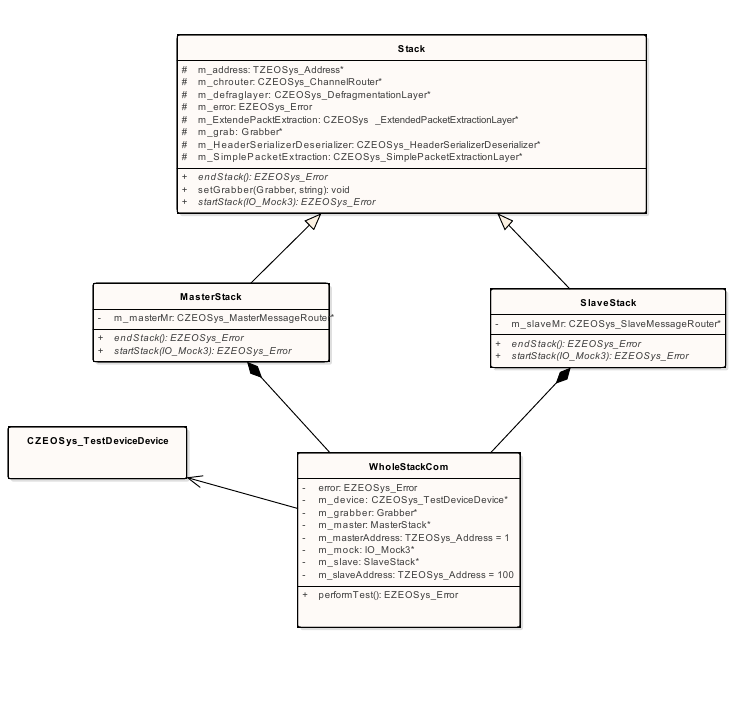
\includegraphics[width=1.0\textwidth]{stack.png}
  \caption{Stack Aufbau}
  \label{fig:Bild3}
\end{figure}


\begin{figure}[htbp] 
  \centering
     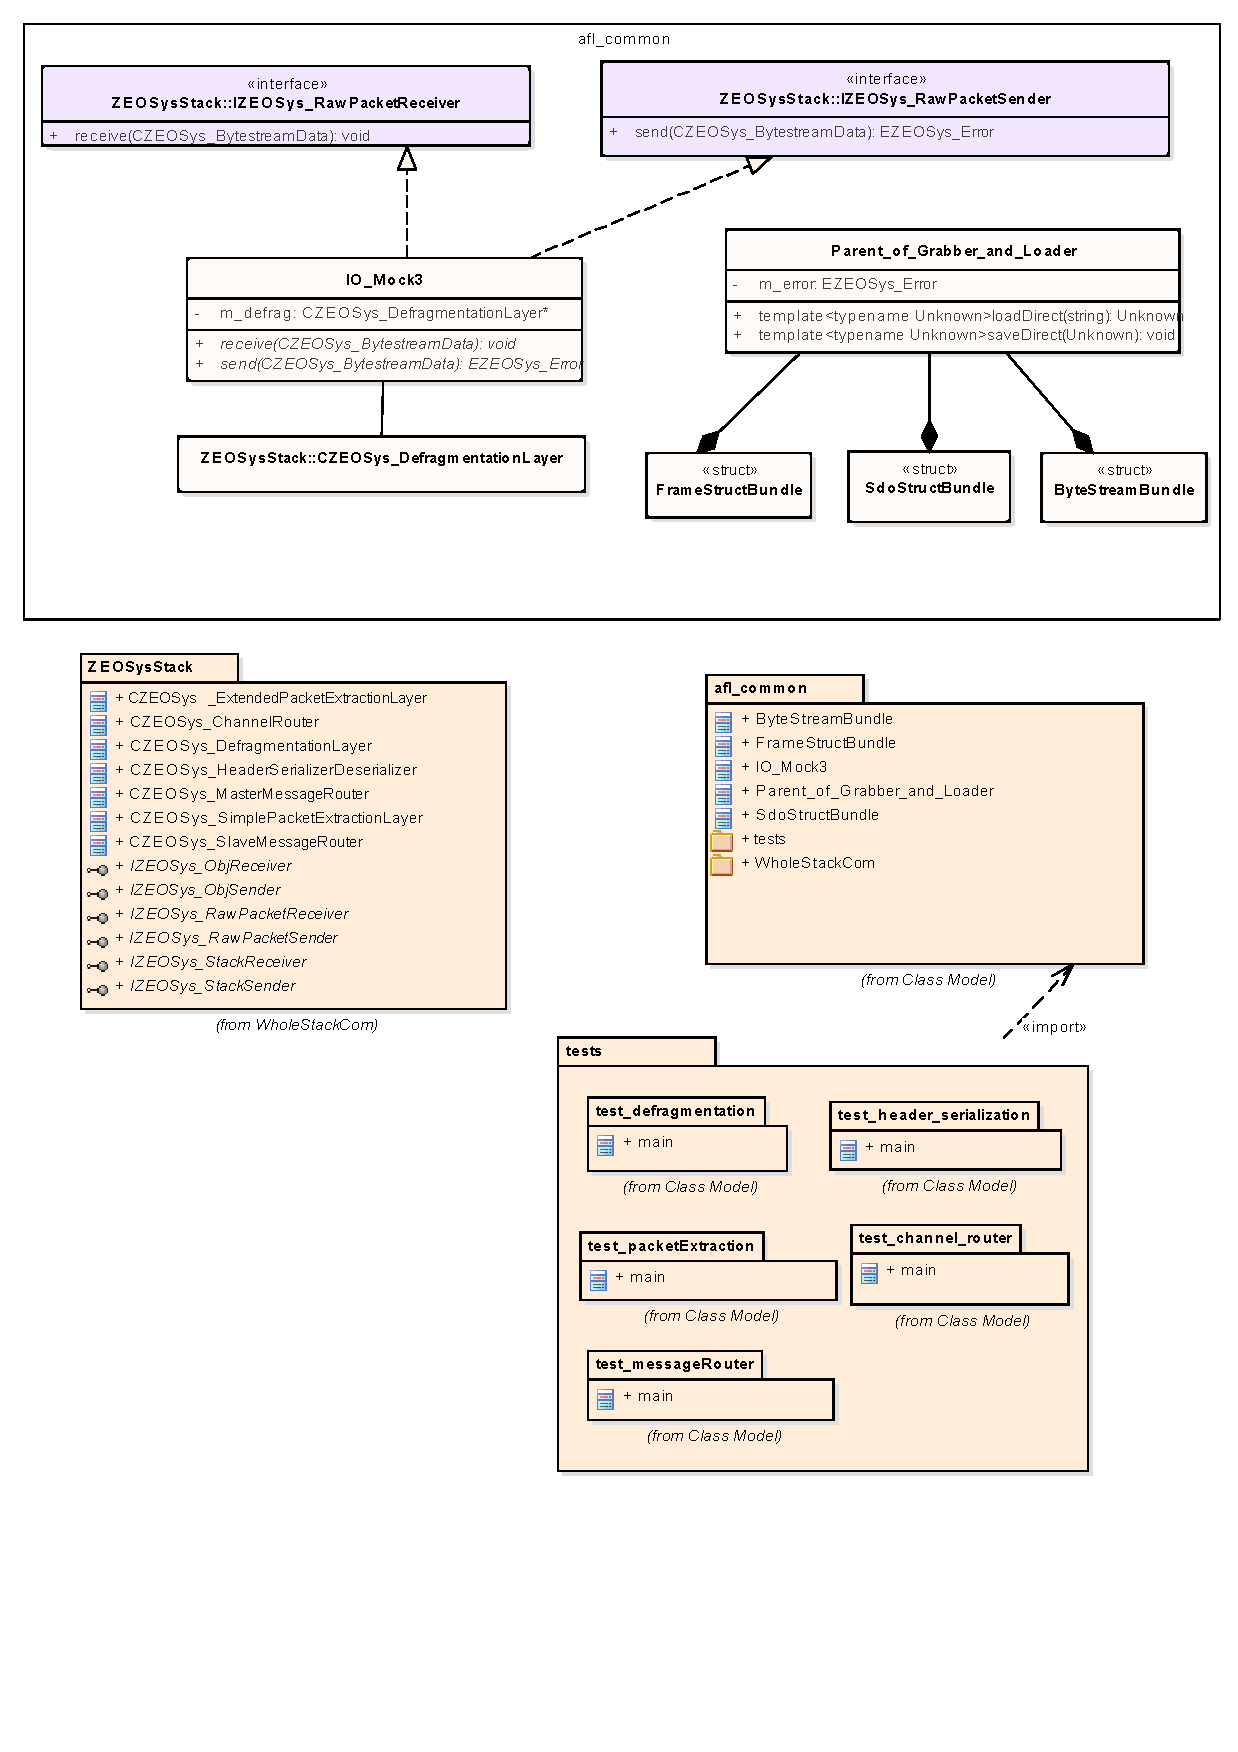
\includegraphics[width=1.0\textwidth]{afl_common.pdf}
  \caption{Paketmodell Testumgebung}
  \label{fig:Bild4}
\end{figure}


% Using typewriter font: \ttfamily inside \lstset
%\begin{frame}

%\lstset{language=C++,
%                basicstyle=\ttfamily,
%                keywordstyle=\color{blue}\ttfamily,
%                stringstyle=\color{red}\ttfamily,
%                commentstyle=\color{green}\ttfamily,
%                morecomment=[l][\color{magenta}]{\#}
%}
%\begin{lstlisting}
%    #include<stdio.h>
%    #include<iostream>
%    // A comment
%    int main(void)
%    {
%    printf("Hello World\n");
%    return 0;
%    }
%\end{lstlisting}
%\end{frame}


\newpage
\section{Auswertung der Testdaten}


\newpage
\chapter{Probleme und Lösungen}

\chapter{Fazit und Zusammenfassung}

\chapter{Quellen}

% https://fuzzing-project.org/tutorial1.html
% http://lcamtuf.coredump.cx/afl/README.txt
% http://lcamtuf.coredump.cx/afl/technical_details.txt
% https://steemit.com/security/@burnin/finding-software- vulnerabilities-by-fuzzing-with-american-fuzzy-lop
%https://en.wikipedia.org/wiki/Fuzzing

\chapter{Abbildungsverzeichnis}
\listoffigures	
	


\end{document}